\chapter{Blockchain}
\texttt{Le informazioni sono state prese dal sito Ethereum.org}\cite{ethereumDocumentiation}
\label{cha:blockchain}

\section{Cos'è?}
Una blockchain è una struttura pubblica, condivisa e immutabile che permette di
salvare dati all'interno di blocchi. I blocchi sono collegati tra loro in modo
tale che ogni blocco verifichi il precedente e per questo modo se un nodo della
catena si rompe, allora tutta la catena viene invalidata.

\section{Parole chiave}
Si usa parola \textbf{blocco} per indicare un insieme di informazioni che
vengono salvate all'interno della blockchain. Infatti i dati non sono inseriti
singolarmente come in un database tradizionale, ma vengono raggruppati in
blocchi di dimensione predefinita e una volta che viene soddisfatta la
dimensione vengono salvati.

Una \textbf{catena} è l'insieme dei blocchi collegati tra loro. Ogni blocco è 
collegato al blocco precedente tramite un codice hash creando in questo modo
un legame inviolabile, dato che la modifica di un blocco porterebbe al 
cambiamento del codice hash e quindi all'invalidazione di tutti i collegamenti
successivi.

Un \textbf{hash code} è l'output risultante da una funzione matematica di
hashing crittografico. Questa funzione prende in input una stringa di lunghezza
variabile e produce un valore di lunghezza fissa. L'output è deterministico,
cioè che per una specifica stringa di input il valore generato sarà sempre lo
stesso. Inoltre, la funzione è unidirezionale, il che significa che è
virtualmente impossibile risalire alla stringa di input originale partendo
dall'output data complessità computazionale di tale operazione, invece è
estremamente semplice passare dall'input all'output in quanto basta applicare
le regole dell'algoritmo. \\
Un algoritmo di hashing ha tra gli obiettivi quello di ridurre il più possibile
la probabilità di collisione accidentale, ossia che due input differenti
restituiscano lo stesso output. Questo evento è molto raro, basti pensare che
il numero possibile di output dell'algoritmo SHA-256 utilizzato da bitcoin è
pari a $2^{256}$. \\ Possiamo distinguere due tipi di funzioni hash:
\textbf{crittografiche} e \textbf{non crittografiche}. Quelle crittografiche
hanno delle peculiarità che le rendono adatte all'uso in blockchain, ad
esempio:
\begin {itemize}
    \item \textbf{Pre-image resistance}: dato un hash code $h$ deve essere
        molto difficile trovare un input $m$ tale che $h = hash(m)$.
    \item \textbf{Second pre-image resistance}: dato un input $m_1$ deve
        essere molto difficile trovare un input $m_2$ tale che $m_1 \neq m_2$
        e $hash(m_1) = hash(m_2)$.
    \item \textbf{Collision resistance}: deve essere molto difficile trovare
        una coppia di input $m_1$ e $m_2$ tali che $m_1 \neq m_2$ e $hash(m_1)
        = hash(m_2)$.
\end {itemize}
Date queste caratteristiche risulta molto complicato sostituire un blocco di una
blockchain con un altro blocco che abbia lo stesso hash in quanto le funzioni
di hash \textit{crittografiche}, a differenza di quelle \textit{non
crittografiche}, mirano a proteggere anche dalla ricerca volontaria di
collisioni e non solo dalle collisioni casuali. 

Ogni computer all'interno della rete è chiamato \textbf{nodo} ed esegue un
software che scarica una copia della blockchain. Il nodo si occupa di validare
i blocchi, si tiene aggiornato sulle transazioni e nuovi blocchi e inoltra gli
aggiornamenti ad altri nodi Questo permette alla tecnologia di essere
distribuita e decentralizzata, in quanto non esiste un server centrale.

Le operazioni che vengono svolte all'interno di questa struttura sono chiamate
\textbf{transazioni} e sono salvate all'interno dei blocchi.

Ora che abbiamo definito le parole chiave, possiamo andare ad analizzare nel 
dettaglio il funzionamento di una blockchain.

\section{Come funziona?}
In questo capitolo andremo ad analizzare il funzionamento di una blockchain,
spiegando i vari passaggi che la contraddistinguono. Prenderemo come
riferimento la blockchain Ethereum in quanto è quella che verrà utilizzata
nell'esempio pratico, tuttavia la maggior parte dei concetti è applicabile 
a tutte le altre blockchain.

\subsection{Transazione}
Una transazione, come detto prima, è un'operazione svolta da un utente
all'interno della blockchain. 

\begin{figure}[H]
    \centering
    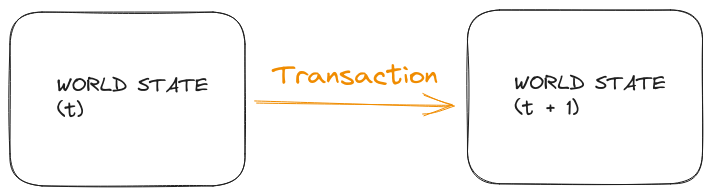
\includegraphics[width=0.7\textwidth]{TransactionSchema.png} 
    \caption{Cambio di stato con transazione}
    \label{fig:transactionSchema}
\end{figure}

Le transazioni che modificano lo stato della struttura devono essere notificate
a tutti gli utenti che vi partecipano. Per fare ciò si utilizza un sistema di
notifiche chiamato \textbf{broadcast} che permette di inviare un messaggio a
tutti i nodi della rete, in questo modo ogni nodo può mandare una richiesta di
esecuzione di una transazione a tutti e in seguito un validatore la eseguirà e
propagherà il cambiamento di stato su tutta la rete. \\
Le transazioni una volta eseguite vengono salvate all'interno di un blocco che
verrà poi aggiunto alla catena.

\subsection{Blocco}
La blockchain è per certi versi simile a un database, ossia il suo scopo è
salvare dati di vario tipo, ma ciò che li differenzia è il modo in cui i dati
vengono salvati. \\ 
Come detto prima la blockchain è una serie di blocchi che contengono
informazioni, in particolare vengono salvati tre dati:
\begin{itemize}
    \item \textbf{Dati}: sono i dati che devono essere salvati. La tipologia di 
        dati può variare in base al tipo di blockchain utilizzata.
    \item \textbf{Hash del blocco precedente}: è l'hash del blocco precedente
        e serve per collegare i blocchi tra loro. Se il blocco precedente viene
        modificato e il suo hash code  cambia, allora non sarà più uguale a
        quello salvato nel blocco successivo e quindi la catena viene
        invalidata.
    \item \textbf{Hash}: è un codice univoco che identifica il blocco e viene
        calcolato in base ai dati contenuti nel blocco stesso. Per poterlo
        calcolare si una appunto una funzione di hashing che prende in input
        i dati e restituisce l'hash.
\end{itemize}

\begin{figure}[H]
    \centering
    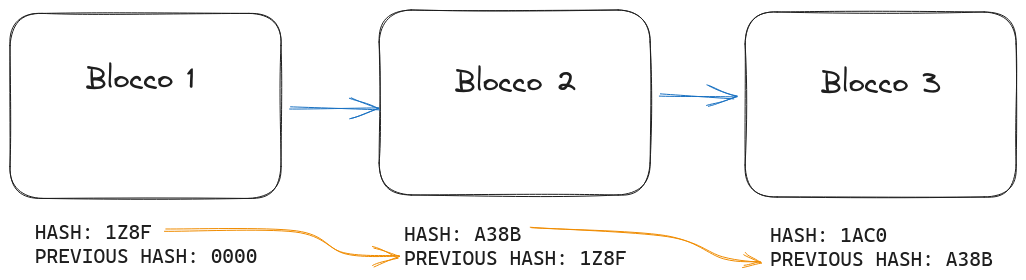
\includegraphics[width=0.9\textwidth]{BlocksSchema.png} 
    \caption{Schema dei blocchi Blockchain}
    \label{fig:chain}
\end{figure}

Dall'immagine precedente \ref{fig:chain} si può notare che ogni blocco
è collegato al blocco prima tramite l'hash del blocco precedente. 
Il primo blocco ha come hash precedente \textit{0000} perchè essendo il blocco
iniziale non esistono blocchi prima di lui.

\begin{figure}[H]
    \centering
    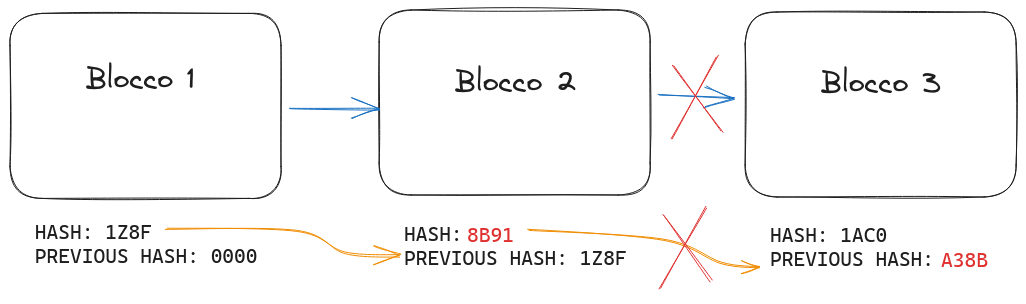
\includegraphics[width=0.9\textwidth]{BlocksSchemaInvalid.png} 
    \caption{Catena invalida}
    \label{fig:invalidChain}
\end{figure}

In questo caso \ref{fig:invalidChain} si può notare che il blocco 2 è stato
modificato e quindi il suo hash code è cambiato. Questo ha portato alla
invalidazione della catena in quanto il blocco 3 non ha più come hash del
blocco precedente quello del blocco 2.

\subsection{Account}
Un account è un'entità all'interno della blockchain che ha un saldo in ETH e
che ha la possibilità di eseguire transazioni. Esistono due tipi di account:
\textbf{Externally-Owned-Account (EOA)} che è un account che può essere gestito
da chiunque abbia la chiavi private e \textbf{Contract Account} che è uno smart
contract all'interno della rete, può essere gestito solo dal codice.

Entrambi i tipi di account possono eseguire operazioni di scambio moneta 
in valuta (ETH) e possono interagire con gli smart contract, ma ci sono delle 
differenze tra i due:

\begin{itemize}
    \item \textbf{EOA:} creare un account non ha un costo e le operazioni che 
        si possono eseguire sono solo transazioni e scambi di ETH. Sono 
        composti da una coppia di chiavi criptografiche, una 
        pubblica e una privata, che permettono di controllare le attività
        dell'account.
    \item \textbf{Contract Account:} la creazione dell'account ha un costo
        in quanto c'è bisogno di caricare il codice dello smart contract
        all'interno della blockchain. Possono eseguire transazioni solo in 
        risposta a richieste ricevute e le azioni eseguite sono quelle definite
        all'interno del codice. Non hanno chiavi come gli account EOA
\end{itemize}

\newpage

Ogni account ha una serie di elementi al suo interno:
\begin{itemize}
    \item \textbf{nonce:} valore che conta il numero di transazioni eseguite
        per un EOA, oppure il numero di contratti creati per un contract
        account. Solo una transazione con un certo nonce può essere eseguito
        da un account, questo aiuta la protezione da attacchi di ripetizione.
    \item \textbf{balance} il numero di ETH che l'account possiede.
    \item \textbf{codeHash:} il codice dell'account che viene anche salvato 
        all'interno della EVM. Non può essere in nessun modo modificato.
    \item \textbf{storageRoot} l'hash code che punta al nodo contenente lo 
        storage per l'account.
\end{itemize}

\begin{figure}[H]
    \centering
    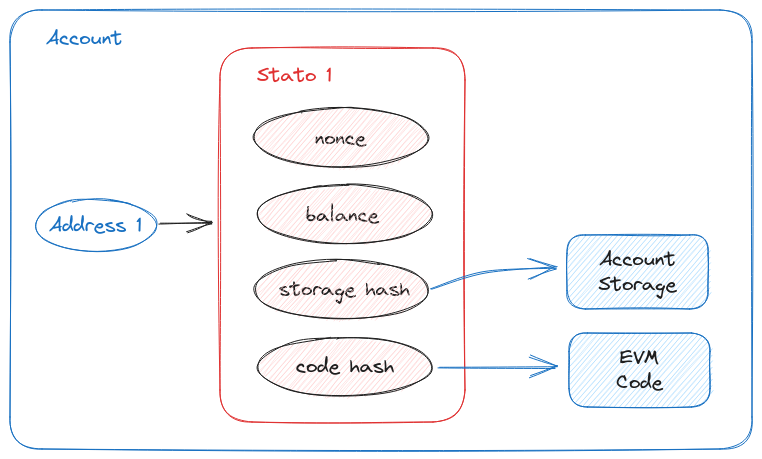
\includegraphics[width=0.9\textwidth]{AccountSchema.png} 
    \caption{Account - \texttt{Ethereum.org}\cite{accountSchema}}
    \label{fig:Account}
\end{figure}

\subsection{Ethereum Virtual Machine (EVM)}
Nella blockchain di Ethereum c'è un solo computer che ha uno stato a cui
ogni partecipante della rete deve fare riferimento. Ogni partecipante ne tiene
una copia e ha inoltre la possibilità di richiedere al computer principale di
eseguire delle operazioni. Quando questa richiesta viene avanzata, altri
nodi della rete si prendono in carico l'operazione e la verificano, validano ed
eseguono notificando poi agli altri ciò che è avvenuto.
Ogni operazione porta al cambiamento dello stato della EVM, e quando ciò
avviene, il nuovo stato viene aggiornato su tutti i nodi della rete. \\
Questo modello di \textbf{macchina a stati distribuita} permette l'esistenza
degli smart contract, ossia dei programmi scritti dagli utenti che possono
essere eseguiti all'interno della blockchain, caratteristica che differenzia
la blockchain di Ethereum da quella di Bitcoin in quanto quest'ultima non
permette l'esecuzione di programmi, limitando di molto le possibilità di
utilizzo della rete.

\begin{figure}[H]
    \centering
    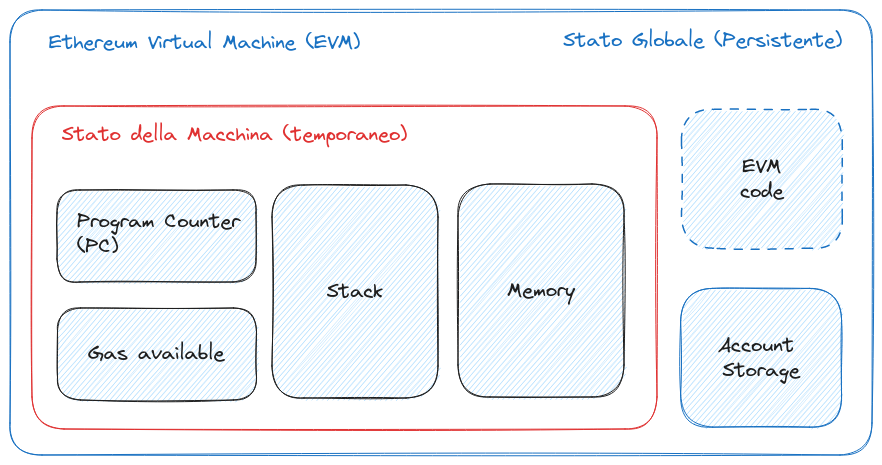
\includegraphics[width=0.9\textwidth]{EVMSchema.png} 
    \caption{Ethereum Virtual Machine - \texttt{Ethereum.org}\cite{EVMSchema}}
    \label{fig:EVM}
\end{figure}

Lo schema \ref{fig:EVM} mostra che la EVM ha uno stato globale che è immutabile
ed è quello su cui tutti devono fare riferimento, ma poi ogni singola macchina
ha il suo stato locale che può essere modificato e poi in caso notificato alle
altre macchine.

Il cambio di stato si comporta come una funzione matematica, ossia dato un
input restituisce un output in modo deterministico. In modo più formale 
possiamo descrivere la funzione come segue:
\begin{equation}
    \label{eq:stateChange}
    S_{t+1} = \Upsilon(S_t, T)
\end{equation}

Dato uno stato $S_t$ e una transazione $T$ viene restituito un nuovo stato
$\S_{t+1}$.

\subsection{Gas fee}
\textbf{Gas} si riferisce all'unità che misura la quantità di sforzo computazionale
richiesto per eseguire operazioni specifiche sulla rete Ethereum. \\
Poiché ogni transazione di Ethereum richiede risorse computazionali per essere
eseguita, tali risorse devono essere pagate per garantire che Ethereum non sia
vulnerabile allo spam e non si blocchi in loop computazionali infiniti. Il
pagamento per la computazione avviene sotto forma di tassa sul gas. \\
\textbf{Gas fee} è la quantità di gas necessaria per eseguire una transazione
moltiplicata per il prezzo di un singolo gas. Il prezzo del gas è espresso in
\textbf{gwei}, che è un sottomultiplo di un ether (1 gwei = $10^{-9}$ ETH).

\textbf{Come vengono calcolate le gas fee?} \\
È possibile impostare la quantità di gas che si è disposti a pagare quando si
invia una transazione. Offrendo una certa quantità di gas, si fa un'offerta per
includere la transazione nel blocco successivo. Se si offre troppo poco, è meno
probabile che i validatori scelgano la transazione per l'inclusione, il che
significa che la transazione potrebbe essere eseguita in ritardo o non essere
eseguita affatto. Se si offre troppo, c'è il rischio di sprecare un po' di ETH.

Il costo totale in gas che si deve pagare è diviso in due parti: 
\textit{base fee} e \textit{priority fee (tip)}. \\
La \textbf{base fee} è la quantità richiesta dal protocollo che bisogna pagare
per poter ritenere l'operazione valida. La \textbf{priority fee} è la quantità
di gas che si offre in più per far eseguire la transazione prima di altre. 

\newpage

Per esempio, se si vuole inviare una transazione che richiede 21.000 gas, la
\textit{base fee} è di 10gwei e si offre 1 gwei come \textit{priority fee},
allora il costo totale sarà: 
\begin{center}
units of gas used * (base fee + priority fee)
\end{center}
\begin{equation}
    \label{eq:gasFee}
    21.000 * (10 + 1) = 0.000021 ETH
\end{equation}

\subsection{Ether}
Abbiamo visto che le gas fee vengono pagate in ETH, ma cos'è l'ETH? \\
\textbf{Ether} (o ETH) è la criptovaluta nativa della blockchain di Ethereum, ciò
significa che gli scambi di moneta all'interno di questa struttura avvengono
con questa valuta. \\
Gli Ether vengono creati come ricompensa per l'azione di proposta e validazione
di un nuovo blocco. L'importo emesso dipende dal numero di validatori e dalla
quantità di Ether che hanno depositato nei loro portafogli digitali. \\
Di solito 1/8 del valore viene destinato a chi ha proposto il blocco e il resto
viene suddiviso tra i validatori. \\
Ovviamente, per evitare il deprezzamento dovuto a inflazione, alcuni Ether 
devono anche essere eliminati, per questo motivo quando un utente effettua
una transazione, la \textit{base fee}, il cui valore viene impostato dalla
rete in base alla domanda, viene eliminata.

\subsection{Meccanismo del consenso}
Il termine meccanismo di consenso si riferisce all'intera serie di protocolli,
incentivi e idee che consentono a una rete di nodi di concordare lo stato di
una blockchain. \\
Ci sono due tipi di meccanismi di consenso: 
\begin{itemize}
    \item \textbf{Proof of Work (PoW)}
    \item \textbf{Proof of Stake (PoS)}
\end{itemize}

\textbf{Proof of Work} \\
Questo meccanismo viene utilizzato all'interno della blockchain di Bitcoin e
veniva utilizzato anche in quella di Ethereum prima del passaggio a Proof of
Stake. Si basa sul concetto di \textbf{mining}, ossia il lavoro svolto per
aggiungere un blocco valido all'interno della catena3 
\begin{itemize}
    \item \textbf{Nuovi blocchi:} I minatori competono per creare nuovi
        blocchi pieni di transazioni elaborate. Il vincitore condivide il nuovo
        blocco con il resto della rete e guadagna alcune criptovalute appena
        coniate (ad esempio BTC nella blockchain Bitcoin). La gara è vinta dal
        computer che riesce a risolvere più velocemente un puzzle matematico e
        la soluzione di questo puzzle è il lavoro di "proof-of-work". Questo
        produce il collegamento crittografico tra il blocco corrente e quello
        precedente. 
    \item \textbf{Sicurezza:} La rete è sicura grazie al fatto che servono il
        51\% della potenza di calcolo totale della rete per poter alterare la
        catena, una quantità di risorse ed energia talmente grande che rende
        assolutamente nulli i possibili benefici di un attacco.
\end{itemize}

\textbf{Proof of Stake} \\
Meccanismo utilizzato in questo momento da Ethereum, in cui i validatori sono
solo nodi che hanno depositato una certa quantità di ETH (in questo momento 32
ETH). 
\begin{itemize}
    \item \textbf{Nuovi blocchi:} I validatori vengono scelti in modo casuale
        basandosi sulla quantità di ETH che hanno depositato. Una volta scelti
        creano un nuovo blocco e lo condividono con il resto della rete,
        ricevendo una ricompensa per il loro lavoro oppure una sanzione
        economica in caso di comportamento scorretto, come ad esempio la
        distruzione di una parte o la totalità degli ETH salvati nel
        portafoglio.
    \item \textbf{Sicurezza:} La rete è sicura perché nel caso un attaccante
        volesse commettere un'azione malevole, metterebbe a rischio gran parte
        dei suoi ETH e quindi molto spesso non è conveniente.
\end{itemize}

\subsection{DAPP (Decentralized Application)}
Una DAPP è un'applicazione sviluppata su una rete decentralizzata che combina 
un frontend con uno smart contract. 

Alcune caratteristiche sono che l'applicazione è:
\begin{itemize}
    \item \textbf{Decentralizzata:} non esiste un server centrale che
        controlla i dati, ma questi sono distribuiti su tutti i nodi della
        rete e quindi sono visibili da tutti.
    \item \textbf{Deterministica:} le operazioni eseguite saranno sempre le
        stesse a prescindere dall'ambiente di esecuzione.
    \item \textbf{Turing completa:} è possibile implementare la macchina di
        Turing, quindi è possibile risolvere qualsiasi problema che ammetta
        soluzione.
    \item \textbf{Isolata:} il codice viene eseguito all'interno della EVM e 
        quindi se un'applicazione è malevola, non può danneggiare il resto del
        sistema.
\end{itemize}

\newpage

Il frontend non differisce in alcun modo rispetto ad una normale applicazione
centralizzata come siamo abituati a conoscere, mentre il backend che è lo smart
contract ha delle peculiarità che analizzeremo nel prossimo capitolo.
Rispetto ad un' applicazione normale, ci sono dei vantaggi e svantaggi che sono
strettamente legati al fatto che il backend sia un algoritmo in blockchain.

\textbf{Vantaggi:}
\begin{itemize}
    \item \textbf{Zero downtime:} una volta che lo smart contract è stato 
        pubblicato sulla rete, sarà sempre disponibile e non potrà essere 
        bloccato da azioni malevole di tipo Denial of Service.
    \item \textbf{Privacy:} non serve fornire dati personali per fare il deploy
        o utilizzare l'applicazione, ma basta avere un portafoglio Ethereum.
    \item \textbf{Resistenza alla censura:} nessuna entità singola può vietare
        ad un utente di effettuare operazioni verso lo smart contract in quanto
        è salvato in blockchain.
    \item \textbf{Integrità dei dati:} i dati sono salvati in blockchain e
        quindi non possono essere alterati da nessuno.
    \item \textbf{Computazione senza fiducia/comportamento verificabile:} I
        contratti intelligenti possono essere analizzati e sono garantiti per
        l'esecuzione in modi prevedibili, senza la necessità di fidarsi di
        un'autorità centrale. Questo non è vero nei modelli tradizionali; ad
        esempio, quando utilizziamo i sistemi bancari online, dobbiamo fidarci
        del fatto che gli istituti finanziari non utilizzino in modo improprio
        i nostri dati finanziari, non manomettano i registri o non vengano
        violati.
\end{itemize}

\textbf{Svantaggi:}
\begin{itemize}
    \item \textbf{Manutenzione:} le dapp possono essere più difficili da
        mantenere perché il codice e i dati pubblicati sulla blockchain sono
        più difficili da modificare. È difficile per gli sviluppatori apportare
        aggiornamenti alle loro dapp (o ai dati sottostanti memorizzati da una
        dapp) una volta che sono state distribuite, anche se vengono
        identificati bug o rischi per la sicurezza in una vecchia versione.
    \item \textbf{Sovraccarico di prestazioni:} c'è un enorme sovraccarico di
        prestazioni e scalare è davvero difficile. Per raggiungere il livello
        di sicurezza, integrità, trasparenza e affidabilità richiesto da
        Ethereum ogni nodo esegue e memorizza ogni transazione ed inoltre anche
        il consenso della proof-of-stake richiede tempo.
    \item \textbf{Congestione della rete:} quando una dapp utilizza troppe
        risorse computazionali, l'intera rete viene sovraccaricata.
        Attualmente, la rete è in grado di elaborare solo circa 10-15
        transazioni al secondo; se le transazioni vengono inviate più
        velocemente di così, il pool di transazioni non confermate può
        rapidamente aumentare.
    \item \textbf{Esperienza dell'utente:} potrebbe essere più difficile
        progettare esperienze user-friendly perché l'utente finale medio
        potrebbe trovare troppo difficile impostare uno stack di strumenti
        necessari per interagire con la blockchain in modo veramente sicuro.
    \item \textbf{Centralizzazione} le soluzioni facili da usare e da
        sviluppare costruite sopra lo strato di base di Ethereum potrebbero
        finire per assomigliare comunque a servizi centralizzati; ad esempio,
        tali servizi possono memorizzare chiavi o altre informazioni sensibili
        sul lato server, servire un frontend utilizzando un server
        centralizzato o eseguire importanti logiche aziendali su un server
        centralizzato prima di scrivere sulla blockchain. La centralizzazione
        elimina molti (se non tutti) i vantaggi della blockchain rispetto al
        modello tradizionale.
\end{itemize}

\newpage

\subsection{Smart Contract}
\label{cha:smart-contract}
Uno smart contract è un programma che gira sulla blockchain di Ethereum. È una
raccolta di \textit{codice} (le sue funzioni) e di \textit{dati} (il suo stato)
che risiede ad un indirizzo specifico sulla blockchain di Ethereum. \\
I contratti intelligenti sono un tipo di conto Ethereum, ciò significa che
hanno un saldo e possono essere oggetto di transazioni, tuttavia non sono
controllati da un utente, ma vengono distribuiti sulla rete ed eseguiti come
programmato. Gli account utente possono quindi interagire con uno smart
contract inviando transazioni che eseguono una funzione definita nello in esso.
Gli smart contract possono definire regole, come un normale contratto,
e applicarle automaticamente tramite il codice e le interazioni con essi sono
irreversibili. \\
Uno smart contract può essere scritto da chiunque tramite i linguaggi di
programmazione \textbf{Solidity} o \textbf{Vyper} e può essere eseguito da
chiunque abbia accesso alla blockchain di Ethereum. \\
La loro principale differenza rispetto a un programma sviluppato per esempio in
Java è che lo smart contract non può accedere a dati che non siano presenti
nella blockchain, quindi non può leggere dati dallo standard input o scrivere
dati sullo standard output, non può effettuare chiamate http o accedere a
database esterni. Questa scelta è stata fatta perché tutti i nodi devono poter
condividere e validare le informazioni, quindi devono essere in grado di
eseguire lo stesso codice e ottenere lo stesso risultato.

Durante il proseguo della tesi verrà utilizzato come linguaggio \textit{Solidity}
per la scrittura degli smart contract. Di seguito un esempio di codice:

\begin{lstlisting}[language=Solidity]
// SPDX-License-Identifier: MIT
pragma solidity ^0.8.0;

contract SimpleStorage {
    string public text;

    function set(string calldata _text) external {
        text = _text;
    }

    function get() external view returns (string memory) {
        return text;
    }
}
\end{lstlisting}

Per il momento non ci interessa sapere a cosa serve ogni componente di questo 
codice, ci basta capire che è un contratto che permette di salvare una stringa
e di leggerla. 

\section{Approfondimento di Solidity}
Per capire meglio i capitoli successivi di questa tesi, è necessario fare un
approfondimento sul linguaggio Solidity, in particolare sulla gestione della 
memoria.

\subsection{Memory e Storage}
Quando vengono dichiarate delle variabili all'interno di uno smart contract, si
può decidere dove salvare i dati, in \textit{memory} o in \textit{storage}, 
questo perchè le operazioni in blockchain hanno sempre un costo e spesso elevato,
qundi questa possibilità aiuta gli sviluppatori a gestire la parte economica
relativa alla scrittura e lettura dei dati. \texttt{}\cite{storageVsMemoryCosts}

\textbf{Storage} \\
I dati persistenti sono rappresentati dalle variabili di stato e questi dati
vengono salvati direttamente sulla blockchain in modo permanente. È neccessario
dichiarare il tipo della variabile in quanto lo smart contract ha bisogno
di sapere quanto spazio allocare in fase di compilazione.
\begin{lstlisting}[language=Solidity]
contract SimpleStorage {
    uint storedData; // State variable
    // ...
}
\end{lstlisting}

\textbf{Memory} \\
Sono i dati temporanei che esistono per la durata dell'esecuzione di una
funzione all'interno dello smart contract. Dato che non vengono salvati in modo
permanente, sono molto più economici da utilizzare rispetto a quelli di stato.

\begin{lstlisting}[language=Solidity]
contract SumCalculator {
    function sum(uint256 _num1, uint256 _num2) public returns (uint256) {
        uint256 memory result = _num1 + _num2;
        return result;
    }
}
\end{lstlisting}

Come si può vedere dal codice, la variabile \textit{result} è stata dichiarata
come variabile di memoria tramite la keyword \textit{memory} e quindi il valore
verrà cancellato non appena la funzione finirà l'esecuzione. 
La parola \textit{memory} in quseto caso poteva anche essere evitata in quanto 
implicita, ma è stata inserita per chiarezza. 

\subsection{Salvataggio dati di grandezza dinamica (Storage)}
Una domanda che può sorgere spontanea è: \textit{Come si fa a salvare dati di
grandezza dinamica in modo permanente?} \\
Se per esempio instanziamo un \textit{mapping} (l'equivalente di un hashmap)
come quello mostrato di seguito, non possiamo sapere a priori quanti elementi
saranno inseriti e quindi non possiamo sapere quanto spazio allocare in fase di
compilazione.

\begin{lstlisting}[language=Solidity]
pragma solidity ^0.8.0;

contract MappingExample {
    mapping(address => uint256) public balances;

    function setBalance(uint256 amount) public {
        balances[msg.sender] = amount;
    }

    function getBalance() public view returns (uint256) {
        return balances[msg.sender];
    }
}
\end{lstlisting}

Ogni smart contract ha accesso alla memoria permanente che può essere pensata
come se fosse un array in cui ogni elemento è di lunghezza \textbf{32 byte} e
l'array ha lunghezza \textbf{2\textsuperscript{256}}. Nonostante questo modello
mentale ci aiuti a capire la grandezza della memoria, dobbiamo ricordare che in
realtà la memoria è sparsa e popolata in modo casuale e il metodo di accesso
utilizza una struttura a \textbf{chiave/valore}. Tutte le celle non utilizzate
sono riempite con uno zero, che a differenza di quello che potremmo pensare,
non occupa nessuno spazio e non serve allocare memoria per esso grazie alla
struttura dati utilizzata che si chiama \textbf{Merkle Patricia Trie}. \\
Ovviamente, per quanto possa sembrare che con uno smart contract si possa 
salvare una quantità di dati praticamente infinita, bisogna ricordare che 
l'aggiunta di ogni dato ha un costo e questo disincentiva all'utilizzo massivo
di questo metodo di storage. \texttt{}\cite{storageSize}

\newpage

\section{Esempio di applicazione nel mondo reale}
La blockchain è una tecnologia che ha preso molto piede negli ultimi anni e 
un esempio pratico di questa espansione lo troviamo nel mondo dell'automotive
con Alfa Romeo. Infatti con il lancio della Alfa Romeo Tonale è stata introdotto
un servizio basato sulla blockchain che permette di registrare tutti i dati del
veicolo per poi creare un certificato che può essere utilizzato come garanzia 
dello stato generale dell'automobile. \\
Questa applicazione dimostra tutti i punti di forza di questa tecnologia, ossia
il fatto che i dati non possano essere modificati e che siano accessibili da
tutti rende il dato salvato nella rete un dato di valore e di fiducia. Inoltre, 
in questo caso specifico vengono anche utilizzati gli \textbf{NFT} che sono
dei certificati digitali sempre basati sulla blockchain che servono appunto
come atto di garanzia rispetto ad un bene, sia fisico che
digitale.\texttt{}\cite{alfaRomeoBlockchain}


